\usetikzlibrary{arrows}

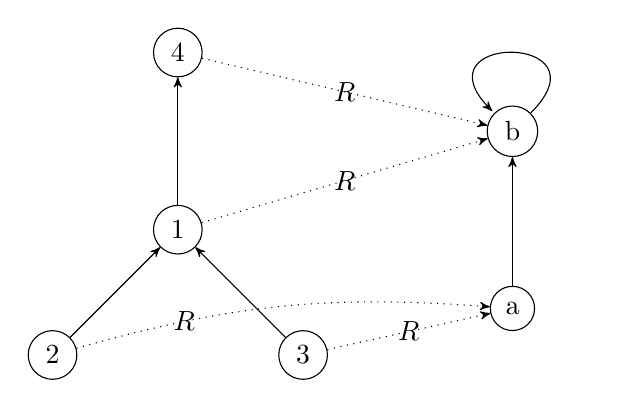
\begin{tikzpicture}[->,>=stealth',node distance=2.25cm]
\node [draw,circle] (1) {1};
\node [draw,circle,below left of = 1] (2) {2};
\node [draw,circle,below right of = 1] (3) {3};
\node [draw,circle,above of = 1] (4) {4};

\node [draw,circle,right of = 1,xshift=2cm,yshift=-1cm] (a) {a};
\node [draw,circle,above of = a] (b) {b};

\path (1) edge (4)
		   (2) edge (1)
		   (3) edge (1)
		   (a) edge (b)
  		   (b) edge [loop] (b)
		   (1) edge [dotted] node {$R$} (b)
		   (4) edge [dotted] node {$R$} (b)
		   (2) edge [dotted,bend left=10] node[near start] {$R$} (a)
		   (3) edge [dotted] node {$R$} (a);
\end{tikzpicture}